\subsection{Project Charter}
The project charter is to be revisited and maintained as the project requirements develop.

\subsection{Product Backlog}
Prioritized list of tasks to be completed. This will be rigorously maintained and updated as the project develops.

\subsection{Sprint Planning}
Sprints are to be voted on and tasks assigned according to each member's skills and preferences.

\subsubsection{Sprint Goal}
As there will be no definitive team manager, the team will vote on goals.

\subsubsection{Sprint Backlog}
The sprint backlog tasks are to be pulled from the highest remaining priority backlog tasks. Lower priority tasks with dependencies will be pulled and assigned as needed.

\subsubsection{Task Breakdown}
The team will vote on each team member's individual tasks every two weeks.

\subsection{Sprint Burndown Charts}
Burndown charts are to be revisited every two weeks.

\begin{figure}[h!]
    \centering
    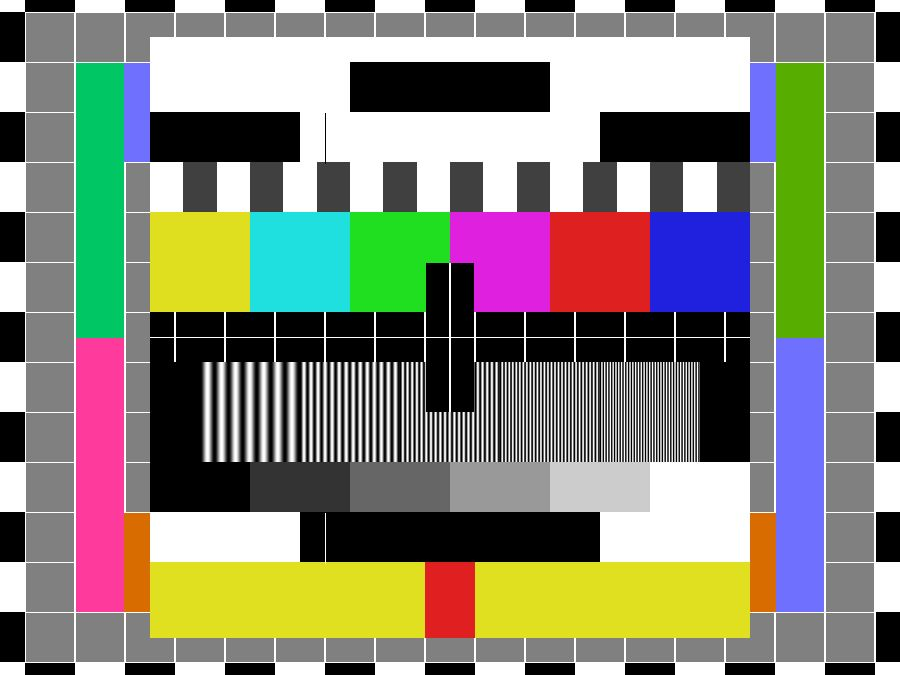
\includegraphics[width=0.5\textwidth]{images/test_image}
    \caption{Example sprint burndown chart}
\end{figure}

\subsection{Sprint Retrospective}
Weekly meetings are in order to discuss the direction of the product development. As development continues, the team will update policies and procedures to ensure maximum working efficiency.

\subsection{Individual Status Reports}
Weekly status reports are to be given by each team member. These may align with the beginning or end of a sprint, or occur mid-sprint.

\subsection{Engineering Notebooks}
The group will have weekly sign offs by team members ensuring that each member's respective work has been documented.

\subsection{Closeout Materials}
Hardware includes the mounted stereoscopic camera set. The group will provide software which allows communication between a PC and a virtual reality headset. Full documentation will be provided. An operational reference guide will be provided for the software needed to run the virtual reality system. A demonstration video is to be provided.

\subsubsection{System Prototype}
No system prototype is available at this point.

\subsubsection{Project Poster}
The team will develop a project poster when the system requirements become more clear.

\subsubsection{Web Page}
The group has agreed against a webpage as it would not serve any practical benefits to the system.

\subsubsection{Demo Video}
A system demonstration video is to be released once a physical prototype is available.

\subsubsection{Source Code}
While the project is software and hardware extensive, there should be nominal source code involved in engineering the system. Team-developed codes will mainly be used to track the gimbal to a virtual reality headset's accelerometer. All source code should remain neat, concise, and efficient.

\subsubsection{Source Code Documentation}
The code's developer should also provide documentation over the code according to standard professional practices.

\subsubsection{Hardware Schematics}
Hardware schematics will be continuously updated as project development continues.

\subsubsection{CAD files}
There will be CAD files which document hardware designs.

\subsubsection{Installation Scripts}
The team will be performing on-site deployment.

\subsubsection{User Manual}
A brief user manual is to be provided which will map the controls relative to the setup of the virtual reality headset and the general warnings associated with virtual reality headset use.
